\section{Criação da empresa} \label{section: Criação da empresa}
\subsection{Introdução}
\par \vspace{8pt}
A Hidden Solutions é uma empresa inovadora no setor das Tecnologias de Informação, especializada no desenvolvimento de soluções tecnológicas focadas na segurança e privacidade digital. Com um forte compromisso com a inovação e a confidencialidade, a Hidden Solutions posiciona-se como um parceiro estratégico para empresas que pretendem transformar e optimizar os seus processos através da digitalização e das mais recentes tecnologias.
\par \vspace{10pt}
Fundada em 2024 por Vladimiro Bonaparte, Lucas Silvestre e João Correia, a Hidden Solutions nasceu com a missão de fornecer soluções tecnológicas personalizadas e eficientes, possibilitanto ás empresas superarem os desafios tecnológicos do mundo moderno. A sua equipa, inicialmente composta por 500 colaboradores, está preparada para crescer de forma sustentada, acompanhando o aumento da procura por soluções digitais de qualidade. Com um capital social de 1.500.000€ e estruturada como uma Sociedade por Quotas (Lda.), a empresa assume uma ambição clara: tornar-se uma referência nacional e internacional no setor, destacando-se pela inovação e pelo compromisso aos seus clientes.
\par \vspace{10pt}
Com especial enfoque no desenvolvimento de software nas áreas de segurança e privacidade, a Hidden Solutions oferece também serviços de consultoria estratégica e apoio à transformação digital. Este vasto leque de soluções permite às empresas adaptarem-se com eficiência ao panorama tecnológico em constante evolução, garantindo ao mesmo tempo a protecção dos seus dados e operações. A empresa está orientada para a criação de valor a longo prazo, comprometendo-se com a satisfação dos seus clientes e o seu sucesso no mercado.
\par \vspace{10pt}
A visão de futuro da Hidden Solutions assenta em consolidar a sua presença no mercado nacional, enquanto se prepara para uma expansão estratégica e célere para o mercado internacional. O seu objetivo é afirmar-se como uma referência global no domínio da segurança digital, oferecendo soluções inovadoras e de confiança, que respondam às exigências de um mundo cada vez mais digital e interligado.
\par \vspace{32pt}
\begin{figure}[H]
    \centering
    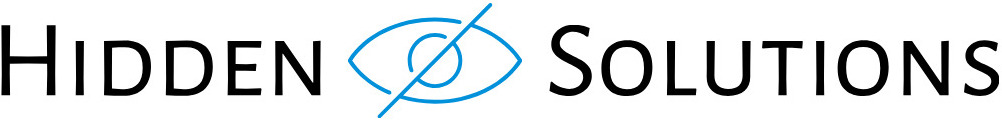
\includegraphics[width=0.8\textwidth]{Figures/0. General/hidden_solutions.jpg}
    \caption{Logotipo da empresa}
    \label{Logotipo da empresa}
\end{figure}

\subsection{Designação e logotipo}
A nossa empresa, Hidden Solutions, foi criada com o objetivo de oferecer soluções inovadoras no campo da segurança e privacidade digital. O nome reflete a nossa missão de proteger as informações sensíveis e resolver problemas que muitas vezes estão ocultos ou passam despercebidos, garantindo a proteção dos dados dos nossos clientes.
\par \vspace{10pt}
O logotipo escolhido, que apresenta um olho parcialmente oculto, simboliza precisamente o foco da empresa em segurança digital. Representa a nossa capacidade de manter a privacidade e proteger os dados dos nossos clientes de forma discreta e eficaz, garantindo que as suas informações estão sempre fora do alcance de ameaças externas. Este design minimalista reflete também a simplicidade e eficiência das nossas soluções, que apesar de complexas a nível técnico, são intuitivas para os utilizadores.
\subsection{Finalidade}